\chapter{Propiedades de los halos}
\label{PropiedadesHalos}


En este capitulo nos enfocamos en el an\'alisis de los halos de materia oscura y sus diferentes propiedades bari\'onicas. Tal como se menciono en la seccion ALGUNA las galaxias en los vac\'ios cosmologicos presentan diferentes caracteristicas respecto a aquellas que habitan ambientes de mayor densidad. Es por esto que es esperable que estas diferencias se manifiesten en cuanto a los halos de materia oscura. Con esto en mente, identificamos los halos de materia oscura en los vac\'ios y realizamos una comparaci\'on entre las propiedades de estos dentro de los voids y en las regiones externas. 

\section{Halos y resoluci\'on}

Para la identificaci\'on de halos en las simulaciones, se utiliz\'o el c\'odigo publico \textbf{\texttt{ROCKSTAR}} \citep{Rockstar} (\textit{Robust Overdensity Calculation using K-Space Topologically Adaptive Refinement} ). El c\'odigo se corre solo sobre las particulas de materia oscura de las simulaciones. El \textit{output} del identificador incluye diversas propiedades de los halos encontrados (como la posici\'on del halo, cantidad de particulas o el radio virial $R_{vir}$), pero no es posible conocer \textit{que particulas} pertenecen a cada halo. 

Para conocer que particulas pertenecen a cada halo, uno puede buscar en la simulaci\'on que particulas se encuentran a una cierta distancia del centro del halo (dato otorgado por \textbf{\texttt{ROCKSTAR}}). Siguiendo esta idea se identificaron las particulas que se encuentren a 2 $R_{vir}$ del halo, construyendo asi halos \'esfericos. De esta manera, se estima la poblacion de particulas de gas, estrellas y materia oscura de los halos. Cabe destacar que la forma real de los halos de materia oscura no es esf\'erica (cita ?), raz\'on por la cual se elige buscar part\'icula mas all\'a del $R_{vir}$. 

Debido a que el identificador \textbf{\texttt{ROCKSTAR}} trabaja solo sobre la materia oscura, hay un sesgo en la masa de los halos que construye. El cat\'alogo de halos que se obtiene con el c\'odigo es de estructuras de al menos 10 particulas de materia oscura, pero como vimos en la secci\'on \ref{SPH} las propiedades de las particulas de SPH se distribuyen sobre una regi\'on que alcanza a la n-esima vecina mas cercana. En el caso de \textbf{\texttt{GIZMO}}, n=56 particulas. De modo que para halos de menos de 56 particulas, la 56-vecina de alguna de las particulas SPH del halo va a estar fuera de este, mientras que para un halo de mas de 56 particulas de SPH la 56-vecina de las particulas de gas va a estar dentro del halo. Este razonamiento va en el sentido de decir que las particulas de gas que pertenezcan a un halo que tenga menos de 56 particulas SPH van a tener parte de su masa fuera del halo. De modo que en este trabajo solo se utilizaron aquellos halos que contengan al menos 56 particulas de gas. (EN REALIDAD FUERON 60 ! )

La figura \ref{PlotControl} presenta la relaci\'on de masa de bariones y materia oscura en funci\'on de la cantidad de particulas de los halos. La l\'inea blanca punteada representa a la fracci\'on cosmologica ($\sim 0.18$. Se puede observar que para halos de pocas particulas la relaci\'on $M_{bar}/M_{dm}$ se aleja mucho de el valor te\'orico cosmologico. \textbf{Esto puede deberse a problemas de resoluci\'on?}. La l\'inea amarilla se\~nala 56 particulas, podemos ver que mas all\'a de este valor la fracci\'on $M_{bar}/M_{dm}$ comienza a parecerse a el valor te\'orico. 



\begin{figure}
    \centering
    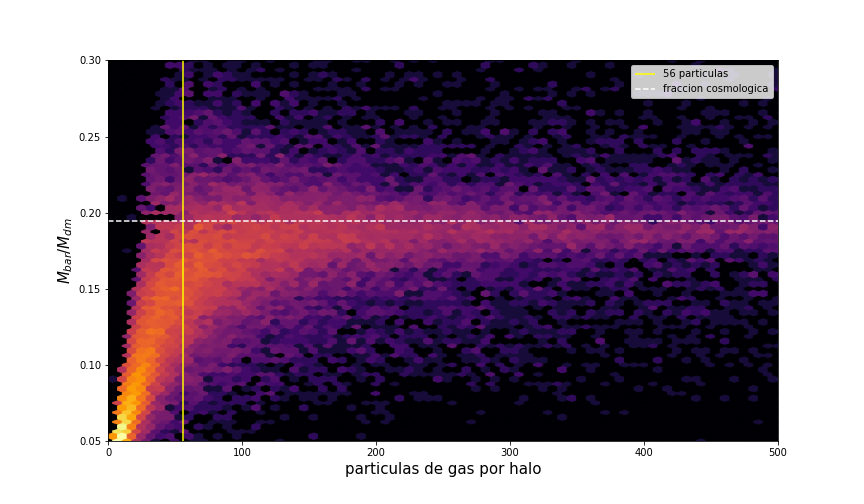
\includegraphics[width=12cm]{Figures/PlotControl.png}
    \caption{Caption}
    \label{PlotControl}
\end{figure}{}


\section{Perfil del Void }

Se explor\'o la posibilidad de que el contenido bari\'onico de los halos de materia oscura tengan alguna dependencia con el entorno, estudiando su distancia al centro del void. Para lo cual se seleccionaron aquellos halos que contengan al menos 56 particulas de gas siguiendo el criterio establecido en la secci\'on anterior y se contruyo el gr\'afico de la figura \ref{PerfilFracciones}.
\begin{figure}
    \centering
    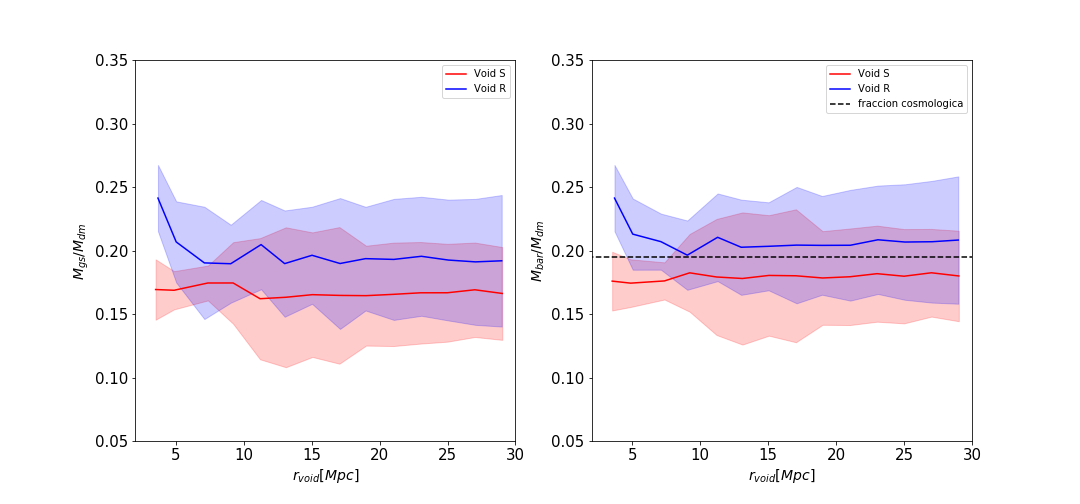
\includegraphics[width=13cm]{Figures/FraccionPerfil.png}
    \caption{Caption}
    \label{PerfilFracciones}
\end{figure}{}
La figura de la izquierda corresponde a la fracci\'on de gas en los halos y la figura de la derecha representa a la fracci\'on de bariones, donde el contenido bari\'onico comprende tanto al gas como las estrellas. Las l\'ineas fueron contruidas teniendo el cuenta la media de cada fracci\'on en cada bin de distancia. La dispersi\'on corresponde a la desviaci\'on est\'andar. 

Si bien la tendencia general es que los halos del void R tengan una fracci\'on mayor de gas o bariones, las diferencias estan contenidas en las dispersi\'ones. En la figura \ref{PerfilFraccionesBar} se presenta la proporsi\'on de estrellas y gas, para halos con al menos una estrella. En este caso la dispersi\'on es demasiado grande y la tendencia no es clara aunque pareciera ser que el void S transformo mas parte de su gas en estrellas, ya que durante la mayor cantidad del perfil tiene una proporsi\'on mayor de estrellas que el void R.  

\begin{figure}
    \centering
    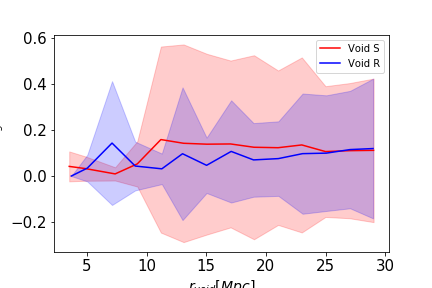
\includegraphics[width=7cm]{Figures/FraccionPerfil_barionic.png}
    \caption{Caption}
    \label{PerfilFraccionesBar}
\end{figure}{}

\section{An\'alisis de regiones}


El prop\'osito de este estudio es identificar que propiedades tienen los halos que pertenezcan a los voids que sean diferentes de las propiedades de halos de entornos mas densos, halos de una regi\'on \textit{homogenea}. Con  esto en mente debemos identificar en nuestras simulaciones alguna regi\'on que pueda ser representativa de un ambiente homog\'eneo. Recurrimos entonces a el contraste de densidad integrado, pero en este caso la integraci\'on se realizara inversamente, es decir, desde \textit{fuera del void} hacia su interior. Definimos entonces:
\begin{equation}
    \Delta_{back}(r)=\int^{in}_{out}\delta(r)dr
\end{equation}{}

Los l\'imites de integraci\'on ser\'an entonces \textit{in}=0 Mpc y \textit{out}=30Mpc. Es importante resaltar que respecto a que hay que tener especial cuidado respecto a el l\'imite externo de integraci\'on (\textit{out}) ya que siempre debemos cuidar de no irnos a regiones tan externas de la simulaci\'on como para contener particulas tidales, ya que como se menciono en la secci\'on ALGUNA estas regiones no estan bien resueltas.

La figura \ref{PerfilesInversos} presenta el contraste de densidad integrado $\Delta_{back}(r)$ desde la regi\'on externa de los voids hacia sus interioriores. De esta manera observamos que en la regi\'on perteneciente a 30-25 Mpc el contraste de densidad es practicamente cero, con lo cual estar\'iamos en una regi\'on \textit{homog\'enea}.

Para seleccionar los halos pertenecientes al void, debemos ir un poco mas all\'a de el radio de cada void. Esto se debe a que la resoluci\'on de las simulaciones realizadas no es suficientemente importante como para obtener una cantidad estad\'isticamente significativa de halos. De modo que debemos relajar un poco el criterio de la definici\'on de void. Clasificamos como halos \textit{del void} aquellos que esten a una distancia tal que $\Delta(r)<-0.7$. Esta condici\'on se cumple a diferentes radios para cada void, siendo entonces $r_{S}=10 Mpc$ y $r_{R}=13 Mpc$.



\begin{figure}[h]
\centering
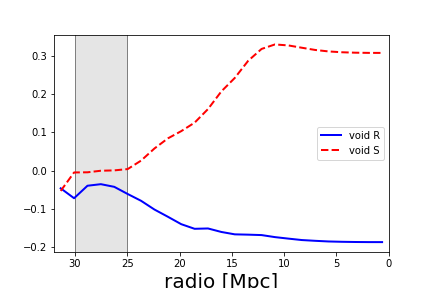
\includegraphics[width=10cm]{Figures/PerfilesInversos.png}
\decoRule
\caption[asd]{}
\label{PerfilesInversos}
\end{figure}

\subsection{Funciones de Masa}




\subsection{Cortes en masa}

Estudiar la dependencia de los halos con el entorno y al mismo tiempo explorar si existe correlaci\'on con la masa de los halos, decidimos separar los halos por bines de masa. De esta manera identificamos los halos realizando 3 cortes indicados en la tabla \ref{CortesMasa}. El criterio para realizar los cortes fue el de mantener significancia estad\'istica. De realizar mas cortes la cantidad de halos en cada uno habr\'ia sido chica como para analizar propiedades globales de las poblaciones.  


\begin{table}[ht]
\begin{tabular}{|l|l|l|l|l|l|}
\hline
  & < 120 particulas  &  120-300 particulas & 300-800 particulas  \\ \hline
S & 48  & 73 &  48              \\ \hline
R & 111  & 92  &    36             \\ \hline
\end{tabular}
\caption{Cantidad de particulas para los halos identificados dentro del void en los diferentes cortes en masa}
\label{CortesMasa}
\end{table}

En la figura \ref{Gs/Dm} presentamos la fracci\'on de masa de gas sobre materia oscura de los halos con los diferentes cortes de masa y diferentes ambientes. Encontramos una tendencia clara en los primeros dos cortes de masa a que los halos de el void S presentan una menor cantidad de gas en relaci\'on a la materia oscura en comparaci\'on al void R. Los halos de fuera de los voids presentan un comportamiento medio entre el de los vac\'ios. Para el tercer corte en masa las distribuciones parecen comportarse similarmente. La l\'inea punteada se\~nala la fracci\'on cosmologica ($\Omega_{bar}/\Omega_{dm}\sim 0.18$). Como en este caso solo estamos mirando las part\'iculas de gas uno podr\'ia pensar que el void S tiene entonces una menor fracci\'on gas/dm debido a que formo estrellas. Para explorar esta idea podemos mirar entonces la fracci\'on bariones sobre materia oscura de los halos.

Las distribuciones de la fracci\'no de bariones sobre materia oscura se presentan en la figura \ref{Bar/Dm} y podemos apreciar que en t\'erminos generales el comportamiento es similar al de la figura \ref{Gs/Dm} donde solo estudiabamos el gas. Esto se debe a que el contenido de estrellas de los halos chicos es insignificante debido a que la resoluci\'on de las simulaciones no alcanza a transformar el gas en estrellas. Con lo cual vemos que los halos de el void S siguen teniendo un menor contenido bari\'onico que los de el R y que los de la regi\'on externa. 

\textbf{MENOS GAS EL VOID S PORQUE TUVO MAS MERGERS. UNA MAYOR TASA DE MERGER VA A HACER QUE EL GAS SE CALIENTE ENTONCES ESTE TENDRA MAYOR TEMPERATURA}


\begin{figure}[h]
\centering
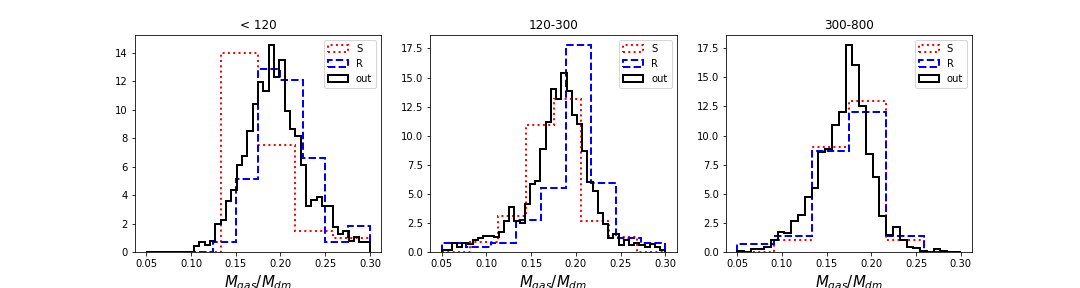
\includegraphics[width=\textwidth]{Figures/Fraccion_cortemasa1.png}
\decoRule
\caption[asd]{Este es fraccion de \textbf{GAS} \textbf{AGREGAR FRACCION COSMOLOGICA}}
\label{Gs/Dm}
\end{figure}


\begin{figure}[h]
\centering
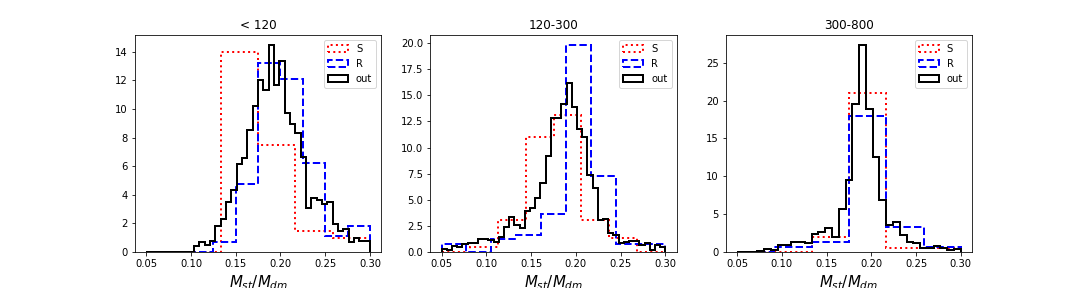
\includegraphics[width=\textwidth]{Figures/Fraccion_cortemasa2.png}
\decoRule
\caption[asd]{Este es fraccion de \textbf{GAS + ESTRELLAS} Entonces las diferencias no se deben a que uno formo mas estrellas que otro. }
\label{Bar/Dm}
\end{figure}


Una propiedad importante para caracterizar el gas es estudiar su temperatura. Podemos asignar una temperatura a un halo considerando el promedio de las temperaturas de gas que lo componen. En la figura \ref{Temperaturas} presentamos la temperatura de los halos. Podemos visualizar una tendencia En las primeras dos regiones (pero fundamentalmente en la primera) a que los halos de el void S estan mas calientes que los halos de el void R, y tambi\'en que los halos de la regi\'on externa. En el tercer corte en masa el comportamiento es contrario ya que la tendencia es que los halos de el void S son mas fr\'ios que los de el R. 


\begin{figure}[h]
\centering
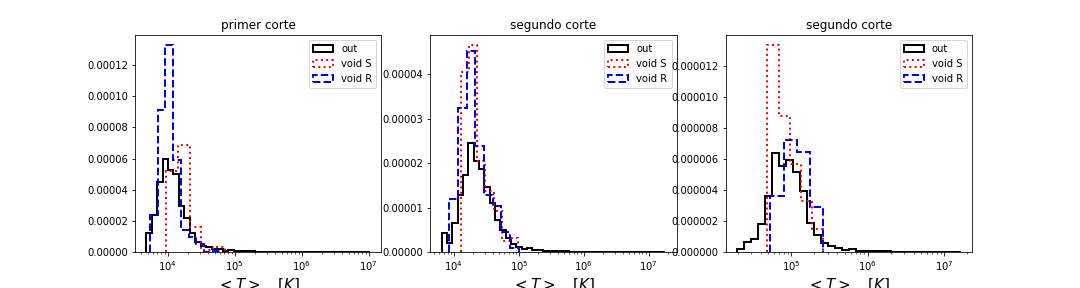
\includegraphics[width=\textwidth]{Figures/temperatura_cortemasa_mean.png}
\decoRule
\caption[asd]{Proba \textbf{sacar el log en el eje y} y meter 11 bines..}
\label{Temperaturas}
\end{figure}

Una posible explicaci\'on para las diferencias encontradas entre el void S y el R en cuanto a la temperatura y contenido de gas de los halos, es que hayan experimentado una tasa de mergers diferentes. Los mergers pueden producir que un halo pierda gas debido a la \textit{ram pressure} \textcolor{red}{\textbf{BUSCAR CITA CLASES HERNAN}} y al mismo tiempo el gas que conserve el halo aumente su temperatura. Debido a que la din\'amica de los voids S y R es fundamentalmente diferente ya que unos se hayan en expansi\'on y otros en contracci\'on, es esperable que la historia de mergers de sus halos sea diferente. \textcolor{green}{Recordemos que las diferencias observadas corresponden a los primeros dos cortes en masa. Mergers de halos grandes son poco probables, lo mas esperable es que los halos grandes \textit{mergen} con halos chicos, pero halos pequen\~os afectaran en menor medida las propiedades de el halo grande, en comparaci\'on a el \textit{merger} de dos halos pequen\~os, y esta podr\'ia ser la raz\'on por la cual no vemos muchas diferencias entre las propiedades de los halos en el tercer corte en masa.}


En la figura \ref{DensCorteMasa} se indica las densidades de gas y materia oscura de los halos $(\rho_{gs}$ y $\rho_{dm}$. Esta densidad es la masa que contiene el halo dividido el radio del mismo (recordemos que los identificamos como 2 $R_{vir}$. Si observamos la densidad de gas, podemos observar una tendencia marginal de los halos del void S a ser mas densos que los halos del void R. Los halos fuera del void pueden alcanzar densidades tanto menores como mayores pero esto se debe a que la muestra es significativamente mayor. No se percibe una tendencia sistem\'atica a un comportamiento caracter\'istico de estos. Al observar la densidad de materia oscura, una comparaci\'on entre los voids para indicar de nuevo que los halos del void S son mas densos que los del R, con la misma salvedad indicada para los halos fuera del void. 






\begin{figure}[h]
\centering
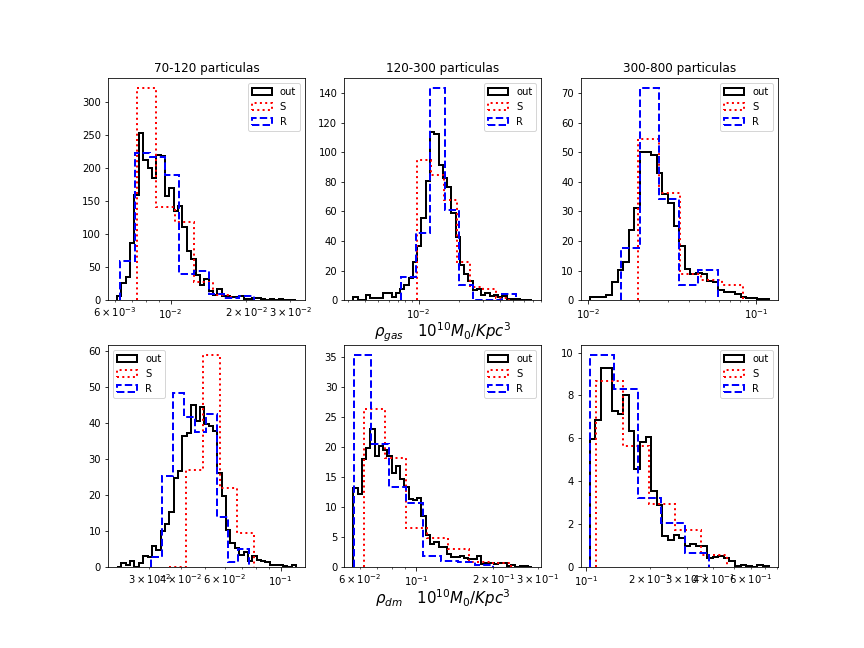
\includegraphics[width=\textwidth]{Figures/Densidades_cortemasa.png}
\decoRule
\caption[asd]{Esta densidad es la cantidad de particulas del halo en 2 radios viriales dividido esta distancia. }
\label{DensCorteMasa}
\end{figure}

Si bien la se\~nal encontrada en la figura \ref{DensCorteMasa} es muy d\'ebil, parecer\'ia indicar que los halos de el void S son m\'as densos que los de el void R, y esto es compatible con lo sen\~alado respecto a que puedade deberse a una diferente historia de \textit{mergers}.



%\begin{figure}[h]
%\centering
%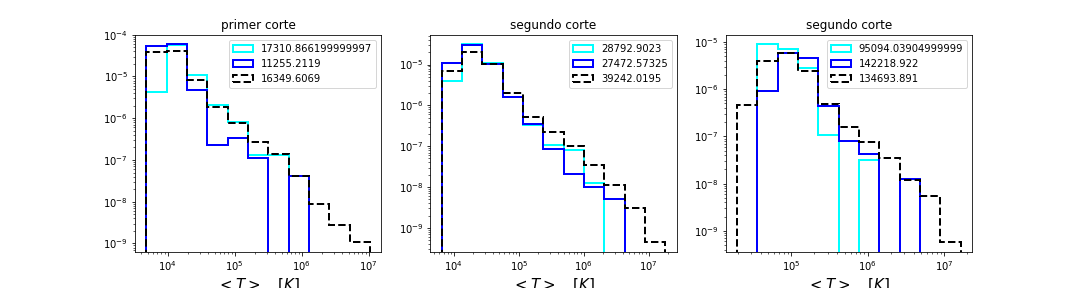
\includegraphics[width=10cm]{Figures/temperatura_cortemasa_median.png}
%\decoRule
%\caption[asd]{}
%\label{fig:Electron}
%\end{figure}


%Para el primer corte
%\begin{tabular}{c|c|c|c|c}
%    - & media & $\sigma/\sqrt{n}$ & mediana & rango cuadratico \\
% \hline   S & 47482.2 & 12608 & 17310& 9036\\
% \hline   R & 47675.3 & 16175 & 11255 & 5170\\
%\hline    U & 166890.1 & 17029  & 16349 &35189.\\

%\hline
%\end{tabular}{}

%Para el segundo corte
%\begin{tabular}{c|c|c|c|c}
%    - & media & $\sigma/\sqrt{n}$ & mediana & rango cuadratico \\
% \hline   S & 96689& 25194 & 28792 & 9036\\
% \hline   R & 89407 & 29988 & 27472 & 5170\\
%\hline    U & 359823 & 26899 & 39242 & 92987\\
%
%\hline
%\end{tabular}{}


%\begin{table}[]
%\begin{tabular}{|l|l|l|l|l|l|}
%\hline
%  & mean                          & $\sigma/\sqrt{n}$ & median & iqs & 92987 \\ \hline
%S & 4.7 $10^{4}$ & 1.3 $10^{4}$            & 0.05   &     &       \\ \hline
%R & 4.7 $10^{4}$ & 1.6 $10^{4}$             & 0.07   &     &       \\ \hline
%U & 1.7 $10^{5}$ & 1.7 $10^{4}$               & 0.06   &     &       \\ \hline
%\end{tabular}
%\end{table}

\section{Entornos Locales}

Un enfoque complementario a lo desarrollado hasta aqu\'i es estudiar el entorno de las estrellas, independientemente de las propiedades de los halos. Si bien todas las estrellas forman parte de halos conceptualmente estamos haciendo algo diferente. 

Estudiaremos entonces el entorno local de las estrellas observando las densidades de materia oscura, gas y estrellas mismas. De esta manera buscamos cuantificar si la formaci\'on estelar en las regiones subdensas presenta caracter\'isticas particulares en comparaci\'on de la contraparte de una mayor densidad. 
 Para realizar esto medimos la distancia a la n-\'esima vecina y utilizamos esta distancia para contruir densidades locales. 

Teniendo en cuenta que tenemos casi 10 veces mas particulas de gas o materia oscura que particulas de estrellas, estimamos las densidades locales utilizando la distancia a la 50-vecina mas cercana para el gas y la materia oscura ($\rho_{gs}$ y $\rho_{dm}$) y la 5-vecina mas cercana para las estrellas ( $\rho_{st}$). Los resultados se presentan en la figura \ref{densidades locales}. Se presentan entonces la densidad de estrellas, gas y materia oscura alrededor de las particulas estelares en nuestra simulaci\'on. 

A la izquierda en la figura \ref{densidades locales} se presenta el entorno estelar. No apreciamos diferencias significativas entre los voids y afuera de estos, aunque pareciera existir una leve se\~nal de que el void R presenta una mayor densidad estelar aunque lejos de ser significativa. 

\begin{figure}
    \centering
    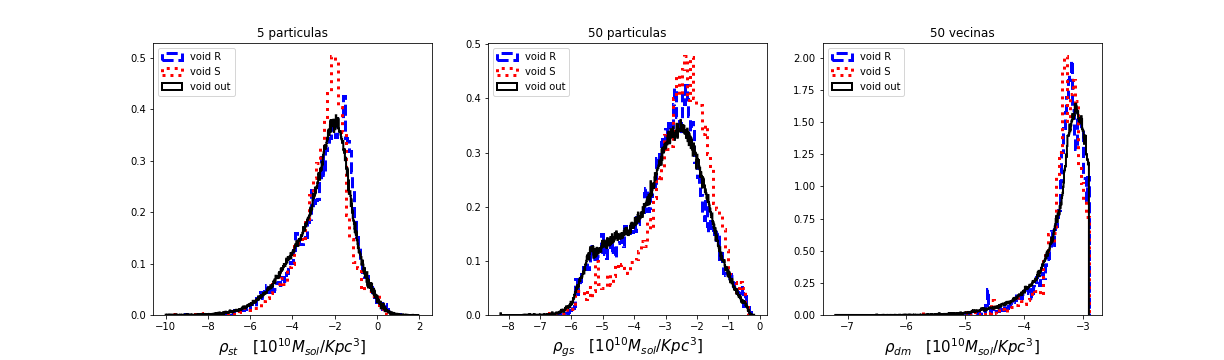
\includegraphics[width=\textwidth]{Figures/densidades_locales.png}
    \caption{Caption}
    \label{densidades locales}
\end{figure}{}

La densidad de gas se presenta en la figura central. Se tiene aqui que el void R y la regi\'on externa se comportan practicamente igual. El caso del void S es mas interesante porque pareciera existir una tendencia a ser mas denso en gas. 

Para estudiar la materia oscura se realiz\'o un corte para eliminar aquellas particulas que presenten una densidad mucho mas all\'a de la longitud de \textit{softening} ($l_{s}$) de la simulaci\'on, ya que a estas escalas tenemos muchas impresiciones en cuanto a la integraci\'on de las particulas. De modo que el corte se realiz\'o en lo que corresponde a una densidad local estimada en un radio de $\sim 1.8 l_{s}$. Tenemos entonces el resultado a la derecha de la figura \ref{densidades locales} donde se observa una leve tendencia en los voids a ser menos densos que la regi\'on externa. Particularmente el void S siendo menos denso que el R. 


El estudio del entorno local aqu\'i representado no es del todo robusto ya que se cuantifica la densidad utilizando una cantidad fija de particulas vecinas y esto no permite estimar la densidad en mas de una escala. Un estudio mas adecuado ser\'ia llevado al cabo utilizando funciones de correlaci\'on, pudiendo de esta manera cuantificar la densidad en una ampl\'ia gama de escalas. 

A\'un bajo estas limitaciones, se observo una tendencia de el void S a tener una mayor densidad de gas alrededor de sus estrellas, lo cual cuadra con lo se\~nalado en la secci\'on anterior ya que como se observo los halos del void S tenian una mayor temperatura. Si el gas se encuentra cercano a las estrellas el \textit{feedback} de estas lo calentara. 

\section{Resumen}
Arranque viendo que los halos del S tiene un mayor contenido de estrellas pesados por masa de gas. Al mismo tiempo en el S tengo menos gas/dm que en el R. Esto lo veo en las fracciones en funcion de los perfiles pero tambien en los primeros dos cortes en masa. Teniendo en cuenta que estan mas calientes y que la densidad de gas alrededor de estrellas es mayor puede deberse a que el feedback calienta el gas y por eos estan mas calientes. Por otro lado, una mayor tasa de mergers pudo por un lado desencadenar procesos de formaci\'on estelar y por otro lado haberle arrancado parte del gas, siendo por esto que tienen menos gas/dm y mas st/gs. (\textbf{aunque el menor st/gs puede ser simplemente porque tiene menos gas...}